\chapter{Wind Turbine Monitoring} \label{s:wt_monitoring}
% First give a short summary of the spectra of different condition monitoring schemes. Importance of predictive maintainance, and \textbf{short summary} of current implementations of predictive maintainance schemes. 

\section{Wind turbine Components}
% Introduce the basic components of a wind turbine, and present some fun statistics about when the different components fail. 
\begin{figure}[h]
    \begin{center}
    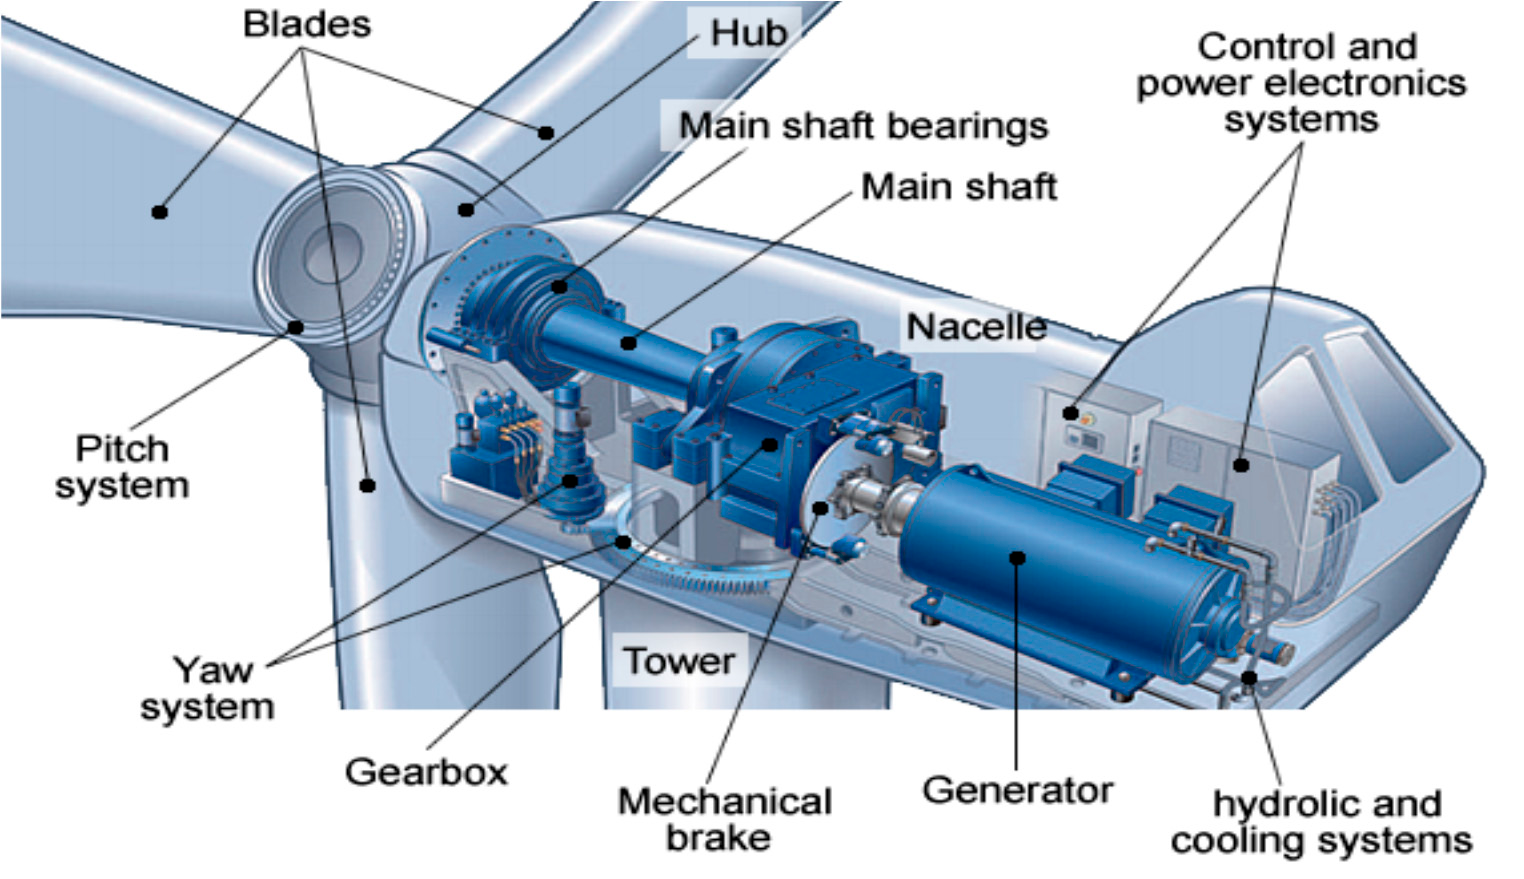
\includegraphics[width=0.8\textwidth]{wind_turbine/wt_parts.png}
    \end{center}
    \caption{Illustration of the different parts of a wind turbine, taken from \cite{adv_meth_for_wt_cond_monit_rev}}
    \label{fig:wt_parts}
\end{figure}

Figure \ref{fig:wt_parts} shows the main parts of a wind turbine which includes the rotor (blades and hub), shafts, gearbox and generator. Simplified a wind turbine works by wind pushing the blades, generating torque that makes the hub rotate. The hub is connected to the gearbox through the main shaft. The gearbox then gears down the torque and gears up the rotational speed to a level that the generator can use to induce current, that goes to a station that transforms the voltage to a level that can be used in the electrical grid. 

\section{Sensors and Data Acquisition}

Information about a wind turbine can come from many sources, it can come from external sources such as images from a camera, or from internal sensors measuring operational data. The collective term for systems measuring operational data is supervisory control and data acquisition (SCADA) systems. To choose what algorithm to use, or what model to use, one must first consider what data one has available. From the literature considered, these where the most used forms of data used as input for the model. 

\begin{itemize}
    \item Vibration measurement  %\cite{wt_bearing_cm_review} \cite{wt_cm_rev_new_trends_chal_2014}
    \item Acustic emission monitoring %\cite{wt_bearing_cm_review} \cite{wt_cm_rev_new_trends_chal_2014}
    \item Temperature measurement %\cite{wt_bearing_cm_review} \cite{wt_cm_rev_new_trends_chal_2014}
    \item Power signal measurement %\cite{wt_bearing_cm_review} \cite{wt_cm_rev_new_trends_chal_2014}
    \item Oil debris monitoring %\cite{wt_bearing_cm_review} \cite{wt_cm_rev_new_trends_chal_2014}
    \item Strain monitoring %\cite{wt_cm_rev_new_trends_chal_2014}
    \item Optical fiber monitoring %\cite{wt_cm_rev_new_trends_chal_2014}
    \item Ultrasonic testing %\cite{wt_cm_rev_new_trends_chal_2014}
    \item Image analysis
\end{itemize}

Analysis of vibration signals is the most common form of condition monitoring used in industry for any form of rotating equipment \cite{wt_bearing_cm_review}. By measuring the acustic emission generated by a component of a wind turbine, one can estimate how much damage it has obtained. The temperature of components in a wind turbine is closely correlated with the health of the component, and is therefore used often in condition monitoring applications \cite{DBN_chicken_swarm_optim}. The power signal can also say a lot about how well a wind turbine is performing, specifically the wind speed - power curve. When monitoring the debris in the oil of a wind turbine gearbox one is analysing the size, type and number of wear particles present in the lubricant, as they can indicate the degree of damage in the gearbox \cite{cm_rnn_lstm}. Strain monitoring, optical fiber monitoring, ultrasonic testing, and image analysis are all used to detect structural damage in different components of the wind turbine, usually the blades \cite{lin_and_non_lin_feat_for_ice_detection_on_blades, image_based_surface_damage_detection_DL_drone_inspection,image_based_YOLO_YSODA, dirt_n_mud_detection_using_guided_waves,blade_defect_detection_imaging_array, unsupervised_AD_blade_damage_deep_features_images}, or tower \cite{wt_cm_rev_new_trends_chal_2014}. The most common approach however was to use a combination of multiple sensors-values to make predictions about the condition about the wind turbine.

\section{Machine learning techniques}
A machine learning is a subset of artificial intelligence. Machine learning models that extract rules from data, which can then be applied to classify, or estimate components of another dataset. Machine learning algorithms are formally divided into \textit{supervised learning}, \textit{unsupervised learning} and \textit{semi-supervised learning}. Supervised learning models require labelled datasets to extract information from the dataset, and are usually used to perform classification tasks, or to estimate a variable that is considered dependent on the input variables (regression). Unsupervised learning algorithms do not require labelled datasets. Semi-supervised learning uses a combination of labelled and unlabelled datasets. \bigskip

% Clustering is a type of unsupervised learning, where the goal is to divide the dataset into clusters, by maximizing some similarity metric for members of the same cluster, and minimizing the same metric for members of different clusters. 

% The use of unsupervised learning methods are not as widespread as the use of supervised learning methods. \textcite{ml_for_wt_cond_monit_rev} only included one article in their review that compared a regression model based on feed forward neural networks to two unsupervised models using gaussian mixture models and self organizing maps. It should be noted that the articles using an unsupervised learning approach that are included in this review, were generally published after \cite{ml_for_wt_cond_monit_rev} was published.

\subsection{Feature extraction}
There are two central problems in condition monitoring that can be solved by feature extraction and selection. The first is the sheer volume of information being produced. A wind turbine with only 20 sensors, sampled at 100 Hz will produce 170 MB of information per day. Feature selection is used here to reduce the number of features to only those relevant for condition monitoring. The second problem is that for systems using only one signal such as vibration, there are many components that are superposed to create the signal that is visible, and there might be noise present. Feature extraction is used to separate the interesting components from each other, and cancel the noise. For some machine learning models feature extraction is not a neccesary preprocessing step, for others careful though must be given as to how to extract features. Table \ref{tab:feat_ext_wt} shows the most frequent methods found in the articles. 

\begin{table*}
    \centering
    \ra{1.3}
    \begin{tabular}{p{0.3\textwidth}p{0.3\textwidth}}
        \toprule
        Articles & Extraction method \\
        \midrule
        ARMA models                         & \cite{ml_cm_wt_blade_ARMA_2018, fault_detection_and_isolation_using_classifier_fusion, lin_and_non_lin_feat_for_ice_detection_on_blades, dirt_n_mud_detection_using_guided_waves, vibration_ARMA_decision_tree_cm_wt} \\
        Discrete Wavelet Transform (DWT)    & \cite{fault_detection_and_isolation_using_classifier_fusion, image_texture_analysis_FD_wt, vibration_acustic_decision_tree_SVM_gearbox, integrated_cm_bearing_fault_wt_gearbox} \\
        Principal Component analysis (PCA)  & \cite{lin_and_non_lin_feat_for_ice_detection_on_blades, multiway_PCA_multivar_inference_cm_wt, dirt_n_mud_detection_using_guided_waves, integrated_cm_bearing_fault_wt_gearbox, unsupervised_AD_blade_damage_deep_features_images, online_fd_using_PCA_different_operating_zones, fault_detect_PARAFAC_k_means}\\
        Basic signal statistics             & \cite{blade_damage_detection_sup_ml_alg, integrated_cm_bearing_fault_wt_gearbox, roller_bearings_cm_fisher_score_and_permutation_entropy} \\
        Neural networks (NN)                & \cite{ice_detection_using_ITL, VMD_MPE_COVAL_fault_detection_gearbox, image_based_surface_damage_detection_DL_drone_inspection, unsupervised_AD_blade_damage_deep_features_images} \\
        \bottomrule
    \end{tabular}
    \caption{Feature extraction and selection methods}
    \label{tab:feat_ext_wt}
\end{table*}

Time-requency domain analysis \cite{fault_detection_and_isolation_using_classifier_fusion, blade_damage_detection_sup_ml_alg}

\subsection{Supervised learning models}
The models that this review considers as supervised learning models, are those only given a dataset which is labelled with fault occurance. The models included in this category are mainly (only?) classification models. 

\subsection{Semi-supervised learning models}